\subsection{Image Classification Setup}

Image Classification Task
    Dataset
    Architecture
    Implementation Details (coding aspect, where it is in the repo, hyperparameters)
    Evaluation
Question Answering System Task
Speech-to-Test Decoding Task




\subsubsection{Dataset}

In this paper we used EMNIST \cite{emnist} data set, which is a collection of handwritten characters and digits from NIST Special Database 19. The data is converted to 28 by 28 matrix so its format matches MNIST data set. There are six subsets in the EMNIST data set: ByClass, ByMerge, Balanced, Letters, Digits and MNIST. We chose the Letter subset because there are around 145k data in it, which will result in a decent running time without loss of information. In the Letter subset, there are 26 classes which corresponding to letter A to letter Z.
\begin{figure}[htp]
    \centering
    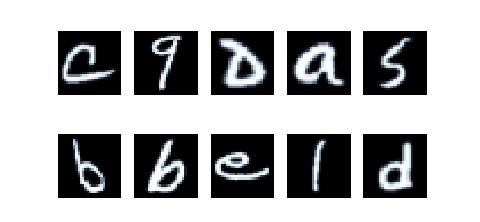
\includegraphics[width=8cm]{img/EMNIST.png}
    \caption{Data instances in EMNIST, which are handwritten 26 alphabetical characters.}
    \label{fig:EMNIST}
\end{figure}



\subsubsection{Evaluation}



The batch size for training is {512, 1024, 2048, 4096, 8192}, the test size is 2048. we keep track of the train loss, test accuracy and test loss for every epoch when using those different optimizers to train the model. For the optimizers, we keep track of the trust ratio and the weight norm of them.


\subsection{Question Answering System Setup}

\subsubsection{Dataset}

For our QA system task, the SQuAD dataset curated by Rajpurkar et al. \cite{squad} is employed. There are 80,000 instances for training and 30,000 instance for testing. For each instance, there are question, answers and the context that the question and answer are based on along with the boundary label of the answer. The task is to read the question in order to (1) retrieve the relevant context and (2) then locate the start and end position of the answer. Example of such an instance is shown in Table \ref{tbl:qasystem}. 

\begin{table}[!b]
\vspace{-5pt}
\scriptsize
\vspace{7pt}
\caption{QA System SQuAD examples. Noted \textit{label} indicating the span of the \textit{answer} inside the context for the corresponding question. }\label{tbl:qasystem}
\vspace{-10pt}
\begin{center}
\begin{tabular}{ l|c|c|l}
 \multicolumn{1}{c|}{Context} &
 \multicolumn{1}{c|}{Question} &
 \multicolumn{1}{c|}{Label} &
 \multicolumn{1}{c}{Answer}\\
 %& & \\
\hline
Architecturally, the  & To whom did the Virgin  & [515,  & St Bernadette 
\\
school has a Catholic...  & Mary allegedly appear... & 541] & Soubirous \\ \hline

Architecturally, the  & What is the Grotto  & [381,  & Marian prayer 
\\
school has a Catholic...  & at Notre Dame? & 420] & \& reflection place \\ \hline

Architecturally, the  & What sits on top of the	  & [92,  & a golden statue 
\\
school has a Catholic...  & Main Building at Notre... & 126] & of the Virgin Mary \\ 

\end{tabular}
\end{center}
\vspace{-15pt}
\end{table}


\subsubsection{Implementation Details}

The first transformation for both the question and the context tokens is that they are passed through an embedding layer initialized with pre-trained GloVe word vectors. 100-dimensional vectors from 6B web crawl version are used here. There are 110K vocabularies in total. For both paragraph and question encoding, we use 2-layer bidirectional LSTMS with $h = 128$ hidden units. Our model is tested on minibatches of 64, 128, 256, and 512. 



\subsubsection{Evaluation}

The model's loss function for updating each batch and epoch is the sum of cross entropy between the predicted and actual of the two tokens. 


\subsection{Speech-to-Text Setup}


% SpeechRecognitionModel(
%   (cnn): Conv2d(1, 32, kernel_size=(3, 3), stride=(2, 2), padding=(1, 1))
%   (rescnn_layers): Sequential(
%     (0): ResidualCNN(
%       (cnn1): Conv2d(32, 32, kernel_size=(3, 3), stride=(1, 1), padding=(1, 1))
%       (cnn2): Conv2d(32, 32, kernel_size=(3, 3), stride=(1, 1), padding=(1, 1))
%       (dropout1): Dropout(p=0.3, inplace=False)
%       (dropout2): Dropout(p=0.3, inplace=False)
%       (layer_norm1): CNNLayerNorm(
%         (layer_norm): LayerNorm((64,), eps=1e-05, elementwise_affine=True)
%       )
%       (layer_norm2): CNNLayerNorm(
%         (layer_norm): LayerNorm((64,), eps=1e-05, elementwise_affine=True)
%       )
%     )
%     (1): ResidualCNN(
%       (cnn1): Conv2d(32, 32, kernel_size=(3, 3), stride=(1, 1), padding=(1, 1))
%       (cnn2): Conv2d(32, 32, kernel_size=(3, 3), stride=(1, 1), padding=(1, 1))
%       (dropout1): Dropout(p=0.3, inplace=False)
%       (dropout2): Dropout(p=0.3, inplace=False)
%       (layer_norm1): CNNLayerNorm(
%         (layer_norm): LayerNorm((64,), eps=1e-05, elementwise_affine=True)
%       )
%       (layer_norm2): CNNLayerNorm(
%         (layer_norm): LayerNorm((64,), eps=1e-05, elementwise_affine=True)
%       )
%     )
%     (2): ResidualCNN(
%       (cnn1): Conv2d(32, 32, kernel_size=(3, 3), stride=(1, 1), padding=(1, 1))
%       (cnn2): Conv2d(32, 32, kernel_size=(3, 3), stride=(1, 1), padding=(1, 1))
%       (dropout1): Dropout(p=0.3, inplace=False)
%       (dropout2): Dropout(p=0.3, inplace=False)
%       (layer_norm1): CNNLayerNorm(
%         (layer_norm): LayerNorm((64,), eps=1e-05, elementwise_affine=True)
%       )
%       (layer_norm2): CNNLayerNorm(
%         (layer_norm): LayerNorm((64,), eps=1e-05, elementwise_affine=True)
%       )
%     )
%   )
%   (fully_connected): Linear(in_features=2048, out_features=500, bias=True)
%   (birnn_layers): Sequential(
%     (0): BidirectionalGRU(
%       (BiGRU): GRU(500, 500, batch_first=True, bidirectional=True)
%       (layer_norm): LayerNorm((500,), eps=1e-05, elementwise_affine=True)
%       (dropout): Dropout(p=0.3, inplace=False)
%     )
%     (1): BidirectionalGRU(
%       (BiGRU): GRU(1000, 500, bidirectional=True)
%       (layer_norm): LayerNorm((1000,), eps=1e-05, elementwise_affine=True)
%       (dropout): Dropout(p=0.3, inplace=False)
%     )
%     (2): BidirectionalGRU(
%       (BiGRU): GRU(1000, 500, bidirectional=True)
%       (layer_norm): LayerNorm((1000,), eps=1e-05, elementwise_affine=True)
%       (dropout): Dropout(p=0.3, inplace=False)
%     )
%   )
%   (classifier): Sequential(
%     (0): Linear(in_features=1000, out_features=500, bias=True)
%     (1): GELU()
%     (2): Dropout(p=0.3, inplace=False)
%     (3): Linear(in_features=500, out_features=29, bias=True)
%   )
% )
% image of the network is the network.png
% https://www.assemblyai.com/blog/end-to-end-speech-recognition-pytorch

\begin{figure}[!t]
    \centering
    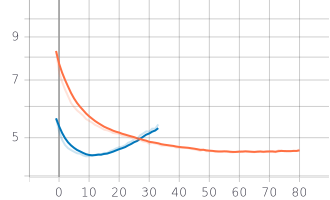
\includegraphics[width=0.7\linewidth]{img/adam_blue_lamb_orange_drqa_256.png}
    \caption{Adam (light blue) and LAMB (orange) test loss convergence graph with batch size of 256.}
    \label{fig:256}
\end{figure}

\subsubsection{Dataset}

Data was preprocessed into spectrograms at a sample rate of 16khz. The task is to map an audio spectrogram frame to one of the 29 output classes (26 alphabet characters, an apostrophe, a space, and an <END> token). 


\subsubsection{Implementation Details}

Residual CNN block includes: 3 layers with 32x32 window size, stride of 2. A fully connected layer from ResCNN to GRU-RNN with 2048 to 500 dimension. Bidirectional GRU-RNN block have three layers with 500 input feature dim and 1000 output features. A final fully connected layer with 1000 input and 500 output. Dropout of 30\%.




\subsubsection{Evaluation}

The model is trained on the Connectionist Temporal Classification (CTC) loss function when aligning audio to transcript, which was originated by \cite{CTC} as shown here for a single (X, Y) pair: 
\begin{center}
$p(Y | X) = \sum_{A\in A_{X, Y}} \prod_t^T = p_t(a_t |. X)$    
\end{center}

CTC first computed the probability for a single alignment step-by-step over multiple sequences then marginalizes over the set of valid alignments to get a distribution over outputs.  